%% What Does JEPA Training Add at Small Scale?
%% Written for the Springer Nature LaTeX template (sn-jnl.cls, option sn-basic).
%% Put this file, sn-bibliography.bib, the figs/ folder and the tables/ folder next to sn-jnl.cls
%% (for example in the Overleaf project created from the "Springer Nature LaTeX Template").

\documentclass[pdflatex,sn-basic]{sn-jnl}% Basic Springer Nature reference style

\usepackage{graphicx}%
\usepackage{multirow}%
\usepackage{amsmath,amssymb,amsfonts}%
\usepackage{amsthm}%
\usepackage{mathrsfs}%
\usepackage[title]{appendix}%
\usepackage{xcolor}%
\usepackage{textcomp}%
\usepackage{booktabs}%
\usepackage{algorithm}%
\usepackage{algorithmicx}%
\usepackage{algpseudocode}%
\usepackage{needspace}%
\usepackage{float}%
\usepackage{capt-of}%

\raggedbottom

\begin{document}

\title[JEPA training at small scale]{What Does JEPA Training Add at Small Scale? Untrained-Encoder Controls and Masking Ablations on CIFAR-10}

% TODO: replace the placeholder name, e-mail and affiliation (add co-authors with \author[1]{...} as needed).
\author*[1]{\fnm{Author} \sur{Name}}\email{author@example.com}

\affil*[1]{\orgdiv{Department}, \orgname{Institution}, \orgaddress{\city{City}, \country{Country}}}

\abstract{Joint-Embedding Predictive Architectures (JEPAs) learn image representations by predicting, in a learned feature space, the content of hidden image regions from the visible ones. Evidence for their design choices, such as the masking strategy or the use of feature-space instead of pixel targets, mostly comes from large models trained once on large datasets, and reported accuracies rarely show how much of a result is due to training rather than to the architecture itself. We study these questions at small scale. We train a 2.7-million-parameter vision transformer with an I-JEPA-style objective on CIFAR-10 and compare it, with paired random seeds, against an untrained encoder with identical initial weights, a pixel-target variant with identical masks and predictor, and three masking strategies (multi-block, single block, random patches). Over three seeds and 50 training epochs, training raises linear-probe accuracy from 34.5\% (untrained) to between 55.2\% and 60.4\%, a gain of 21 to 26 percentage points. Replacing feature-space targets by normalised pixel targets did not lower linear-probe accuracy (difference $-0.2 \pm 2.4$ points for multi-block masking), although feature-space targets were ahead on $k$-nearest-neighbour accuracy ($+3.8 \pm 3.0$). Multi-block masking outperformed random-patch masking by $3.7 \pm 2.9$ points, whereas single-block and multi-block masking could not be told apart. No configuration showed representation collapse. The study is limited to one dataset, short training and three seeds; code and all results are public.}

\keywords{JEPA, self-supervised learning, masked prediction, ablation study, CIFAR-10}

\maketitle

%% ------------------------------------------------------------------------------------------
\section{Introduction}\label{sec:intro}

Learning useful representations of images and video without human labels is a central goal of machine learning, and it is closely tied to the idea of a world model: a system that learns how its environment is structured and how it changes~\cite{ha2018worldmodels,lyu2026survey}. Joint-Embedding Predictive Architectures (JEPAs) are a family of self-supervised methods built around this idea. Instead of reconstructing the missing parts of an input pixel by pixel, a JEPA predicts a \emph{representation} of the missing parts, computed by a slowly updated copy of the encoder, from the parts that are visible. The image version, I-JEPA~\cite{assran2023ijepa}, has been followed by variants for motion and content~\cite{bardes2023mcjepa}, dense video features~\cite{murlabadia2026vjepa21}, vision--language modelling~\cite{chen2025vljepa}, object-level world models~\cite{nam2026cjepa} and planning~\cite{zhang2026hierarchical,destrade2025value}; see also the tutorial of Monemi et al.~\cite{monemi2025tutorial}.

Three things make it hard for a newcomer to know what to take away from this literature. First, the accuracy of a trained model does not show how much of that accuracy was \emph{added by training}. Even a network with random weights produces features that are far better than chance~\cite{saxe2011random}, and for a vision transformer evaluated on frozen features the untrained architecture already retains a good deal of image information. A reference point is therefore needed, and the natural one is the same network before training. Second, design choices such as the masking strategy and the choice of feature-space rather than pixel targets are usually ablated once, at large scale, with a single reported number per setting. When two recipes differ by a few points, it is not clear whether the difference exceeds the variation between random seeds. Third, most readers cannot repeat large-scale experiments, whereas a small version of the same recipe can be repeated many times.

In this paper we run such a small version. We train an I-JEPA-style model on CIFAR-10 and ask three questions.
\textbf{RQ1:} how much of the accuracy of a small JEPA encoder comes from training, as opposed to its untrained architecture?
\textbf{RQ2:} in this setting, does predicting feature-space targets beat predicting normalised pixels?
\textbf{RQ3:} does the masking strategy matter, and are the differences larger than seed-to-seed variation?
We also check, as a side question, whether any configuration suffers representation collapse, and whether the training loss tells us which recipe is better.

Our contributions are the following. First, a paired experimental design: for each random seed, the untrained encoder and every trained model start from identical weights, so the effect of training is measured as a paired difference with a confidence interval. Second, empirical answers to RQ1--RQ3 over three seeds, including a pixel-target control with identical masks and predictor, reported together with the places where the data are inconclusive. Third, a short, resumable implementation that reproduces all 18 runs in about an hour on one consumer GPU, released with the raw results.

This is not a new method, and it is not a state-of-the-art result. It is a controlled, small-scale study of an existing recipe, and its conclusions should be read as such. The rest of the paper is organised as follows: Section~\ref{sec:related} reviews related work and the gap we address, Section~\ref{sec:methods} describes the experimental design, Section~\ref{sec:results} reports the results, Section~\ref{sec:discussion} discusses them and their limits, and Section~\ref{sec:conclusion} concludes.

%% ------------------------------------------------------------------------------------------
\section{Background and related work}\label{sec:related}

\subsection{The JEPA idea}\label{sec:jepa-idea}
A JEPA uses three networks. A \emph{context encoder} reads the visible part of an input. A \emph{target encoder}, which has the same architecture and whose weights are an exponential moving average of the context encoder's weights, reads the whole input and produces the targets. A \emph{predictor} receives the context encoder's output together with the positions of the hidden regions and predicts the target encoder's output at those positions. The training loss compares prediction and target in feature space. Because the targets come from a slowly changing copy of the encoder, and not from a fixed external signal, such methods can in principle collapse to a trivial constant representation; self-distillation methods such as BYOL~\cite{grill2020byol} and DINO~\cite{caron2021dino} use moving-average targets, together with other safeguards, to avoid this. In I-JEPA~\cite{assran2023ijepa} the input is an image divided into patches, the context is a large block of patches, and the targets are several smaller blocks. By contrast, masked autoencoders~\cite{he2022mae} also hide patches but reconstruct their pixels.

\subsection{Existing evidence on masking and targets}\label{sec:evidence}
The I-JEPA paper reports two ablations that are directly relevant to us. For the masking strategy, using a ViT-B/16 trained for 300 epochs and a linear probe on 1\% of the ImageNet-1K labels, its multi-block strategy reaches 54.2\% top-1 accuracy, compared with 15.5\% for rasterised masking, 20.2\% for a single block and 17.6\% for random patches~\cite{assran2023ijepa}. For the targets, predicting target-encoder outputs reaches 66.9\% and predicting pixels 40.7\% in the same 1\%-label protocol, with a ViT-L/16 and different numbers of epochs (500 and 800)~\cite{assran2023ijepa}. These are large effects at large scale, with one number per setting and no intervals shown. A recent theory of JEPA world models connects pretraining error to planning regret and predicts an approximation--sample trade-off governed by the latent dimension, with implications for latent-level versus input-level prediction~\cite{cui2026theory}. A vision--language JEPA has also been compared with token-space training under controlled conditions~\cite{chen2025vljepa}.

\subsection{Controls and diagnostics}\label{sec:controls}
Random-weight networks have long been used to separate the contribution of architecture from that of learning~\cite{saxe2011random}. A second common concern in self-supervised learning is representation collapse, in which features lose variety. A widely used diagnostic is the effective rank of the feature matrix~\cite{garrido2023rankme}, which we use in a mean-centred form.

\subsection{The gap}\label{sec:gap}
To our knowledge, the JEPA studies we surveyed do not report an untrained encoder as a reference for their linear-probe numbers, and their ablations are given as single runs. We cannot rule out that such controls exist elsewhere, and we do not claim priority; our aim is to make the untrained control, a pixel-target control and seed-to-seed variation the \emph{focus} of a study rather than a footnote, in a setting small enough to be repeated.

%% ------------------------------------------------------------------------------------------
\section{Experimental design}\label{sec:methods}

\subsection{Data}\label{sec:data}
We use CIFAR-10~\cite{krizhevsky2009cifar}: 50,000 training and 10,000 test colour images of $32\times 32$ pixels in 10 classes. A fixed random subset of 5,000 training images (the same for every run) is held out as a validation set; the remaining 45,000 images, without their labels, are used for pre-training. Images are normalised by the per-channel mean and standard deviation of the 45,000 pre-training images. During pre-training only, we apply random crops (4-pixel reflection padding) and horizontal flips. No augmentation is used at evaluation time.

\subsection{Model}\label{sec:model}
Figure~\ref{fig:arch} shows the architecture. The encoder is a small vision transformer (ViT)~\cite{dosovitskiy2021vit}: the image is split into $8\times 8=64$ non-overlapping patches of $4\times 4$ pixels, each patch is linearly embedded to 192 dimensions and combined with a fixed two-dimensional sine--cosine position embedding, and the tokens pass through 6 pre-norm transformer blocks (3 attention heads, MLP ratio 4) followed by a layer normalisation. It has 2.68 million parameters. The predictor is a narrower transformer (width 96, 4 blocks, 3 heads, 0.48 million parameters): it linearly projects the context tokens to width 96, appends one learned mask token per target position (with that position's embedding added), applies its blocks, and maps the outputs at the target positions back to the target dimension. The target encoder is a copy of the encoder whose weights are not trained by gradient descent.

\begin{figure}[t]
\centering
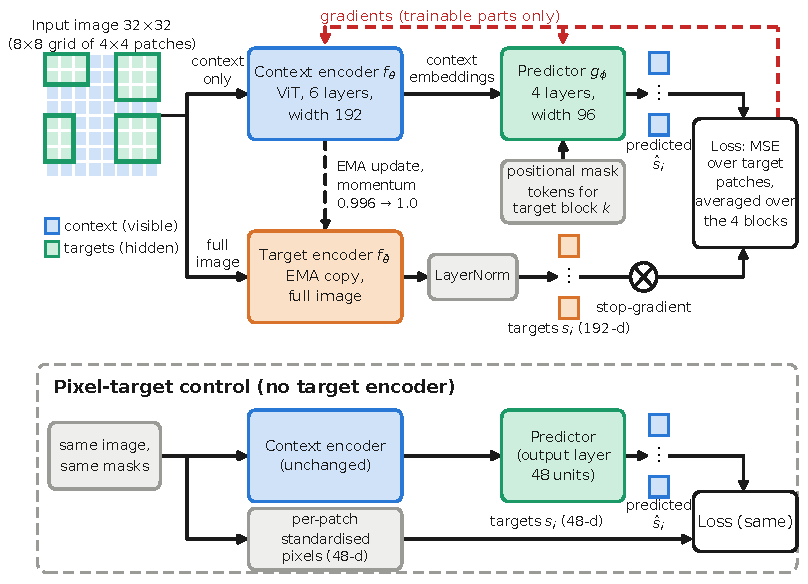
\includegraphics[width=\textwidth]{figs/fig_architecture.pdf}
\caption{Training set-up. The context encoder sees only the context patches. The target encoder, an exponential moving average of the context encoder, sees the whole image; its layer-normalised outputs at the target positions are the regression targets. The predictor receives the context features and one mask token per target position and predicts the targets. The loss is the mean squared error between predictions and targets, and gradients flow only through the context encoder and the predictor. In the pixel-target control, the target encoder is replaced by per-patch normalised pixel values.}\label{fig:arch}
\end{figure}

\subsection{Training objective}\label{sec:objective}
Let the image have $N=64$ patches, let $C$ be the set of context positions and $T_1,\dots,T_K$ the target blocks. Write $f_\theta$ for the context encoder, $f_{\bar\theta}$ for the target encoder and $g_\phi$ for the predictor. The target at position $i$ is the layer-normalised target-encoder output $s_i=\mathrm{LN}\big(f_{\bar\theta}(x)\big)_i\in\mathbb{R}^{192}$, computed from the full image without gradients. For each target block $T_k$ the predictor outputs $\hat s^{(k)}_i = g_\phi\big(f_\theta(x_C), C, T_k\big)_i$ for $i\in T_k$, and the loss is
\begin{equation}
\mathcal{L}=\frac{1}{K}\sum_{k=1}^{K}\frac{1}{|T_k|\,d}\sum_{i\in T_k}\big\lVert \hat s^{(k)}_i - s_i\big\rVert_2^2 ,
\label{eq:loss}
\end{equation}
with $d=192$. After each optimiser step the target encoder is updated by $\bar\theta\leftarrow m_t\bar\theta+(1-m_t)\theta$, where $m_t$ increases linearly from 0.996 to 1.0 over training. One training step is summarised in Algorithm~\ref{alg:step}.

In the \emph{pixel-target} control there is no target encoder. The target at position $i$ is the vector $u_i\in\mathbb{R}^{48}$ of the (normalised, augmented) pixels of patch $i$, standardised within the patch to zero mean and unit variance, $s_i=(u_i-\bar u_i)/\sqrt{\mathrm{var}(u_i)+10^{-6}}$. The masks, encoder and predictor are unchanged except that the predictor's output layer has 48 outputs; Equation~\ref{eq:loss} holds with $d=48$.

\begin{algorithm}[t]
\caption{One training step (feature-space targets).}\label{alg:step}
\begin{algorithmic}[1]
\Require batch of images, encoder $f_\theta$, target encoder $f_{\bar\theta}$, predictor $g_\phi$, masking strategy, momentum $m_t$
\State $x \gets$ augment(normalise(batch))
\State sample context positions $C$ and target blocks $T_1,\dots,T_K$ (Section~\ref{sec:masking})
\State $s \gets \mathrm{LN}\big(f_{\bar\theta}(x)\big)$ \Comment{full image, no gradient}
\State $z \gets f_\theta(x_C)$ \Comment{context patches only}
\For{$k = 1,\dots,K$}
  \State $\hat s^{(k)} \gets g_\phi(z, C, T_k)$
\EndFor
\State $\mathcal{L} \gets \frac{1}{K}\sum_k \mathrm{MSE}\big(\hat s^{(k)}, s_{T_k}\big)$
\State update $\theta,\phi$ by one AdamW step (gradient-norm clipping at 1.0)
\State $\bar\theta \gets m_t\bar\theta + (1-m_t)\theta$
\end{algorithmic}
\end{algorithm}

\subsection{Masking strategies}\label{sec:masking}
We compare three strategies on the $8\times 8$ patch grid (Table~\ref{tab:masks}). \emph{Multi-block} follows I-JEPA: four target blocks, each covering 15--20\% of the grid with aspect ratio between 0.75 and 1.5, and one context block covering 85--100\% of the grid from which all target patches are removed. One block shape is drawn per batch and positions are drawn per image, and the context is truncated to the smallest context in the batch (at least 10 patches). \emph{Single block} hides one $4\times 4$ block (25\% of the patches) at a random position, and the context is everything else. \emph{Random patches} hides 16 randomly chosen patches (also 25\%), and the context is everything else.

\begin{table}[t]
\caption{Masking strategies. Patch counts per image are measured by simulating 2,000 batches of 256 images with the code used in the experiments. Target counts for multi-block are summed over the four blocks, which may overlap.}\label{tab:masks}
\begin{tabular}{@{}lccc@{}}
\toprule
Strategy & Target blocks & Target patches & Context patches\\
\midrule
Multi-block & 4 blocks, 15--20\% of grid each & 32--48 (mean 43.4) & 10--19 (mean 12.1)\\
Single block & 1 block, $4\times4$ & 16 & 48\\
Random patches & 16 scattered patches & 16 & 48\\
\botrule
\end{tabular}
\end{table}

Single-block and random masking hide the same number of patches and leave the same context size, so they differ only in whether the hidden patches are contiguous. Multi-block masking differs from both in the amount of visible context and in the number of targets, which we return to in Section~\ref{sec:discussion}.

\subsection{Conditions}\label{sec:conditions}
We run six conditions: (i)~\texttt{raw\_pixels}, a classifier on the normalised pixel vector (3,072 dimensions), with no network; (ii)~\texttt{untrained}, the encoder at initialisation; (iii)~JEPA with multi-block masking; (iv)~JEPA with single-block masking; (v)~JEPA with random-patch masking; and (vi)~the pixel-target control with multi-block masking. Conditions (iii)--(vi) are trained for 50 epochs. The training hyperparameters (Appendix~\ref{app:hparams}) follow the I-JEPA recipe scaled down to this setting, and were \emph{not} tuned for any condition.

\subsection{Evaluation protocol}\label{sec:eval}
After training, the encoder is frozen. For each image we pass all 64 patches through it (no masking, no augmentation) and average the 192-dimensional output over the patches. We evaluate with two classifiers on these features.

\paragraph{Linear probe.} Features are standardised with the mean and standard deviation of the labelled training subset used for that probe, and a linear classifier is trained with Adam (learning rate 0.01, cosine schedule, 300 full-batch steps) on cross-entropy plus an $\ell_2$ penalty on the weights. The penalty strength is chosen from $\{10^{-5},\dots,10^{-1}\}$ by accuracy on the validation set; the test set is then scored with the selected classifier. We train probes on 100\%, 10\% and 1\% of the 45,000 labelled training images (45,000, 4,500 and 450 images); the subsets are drawn at random with the run's seed, so every condition with the same seed uses the same subset.

\paragraph{$k$-nearest neighbours.} Each test image is classified by a similarity-weighted vote ($k=20$, cosine similarity, temperature 0.07) among the 45,000 training features.

\paragraph{Collapse diagnostic.} On the features of the validation images we compute the effective rank of the mean-centred feature matrix, $\exp\!\big(-\sum_j p_j\ln p_j\big)$ with $p_j=\sigma_j/\sum_l\sigma_l$ and $\sigma_j$ the singular values~\cite{garrido2023rankme}. It is at most 192 here and approaches 1 when the features collapse to a single direction.

We evaluate at epochs 0, 25 and 50 (epoch 0 is the untrained encoder with the run's seed). We report the final epoch; no checkpoint is selected using test data.

\subsection{Seeds, pairing and statistics}\label{sec:stats}
Every condition is run with seeds 0, 1 and 2. For a given seed, the untrained encoder and all trained models start from identical weights, so that the effect of training, and the differences between recipes, are measured as \emph{paired} differences across seeds. We report means with 95\% confidence intervals based on the $t$-distribution with two degrees of freedom (critical value 4.30). With only three seeds these intervals are wide and approximate. We report 24 paired comparisons (8 pairs of conditions, 3 metrics) without correction for multiple testing; with 95\% intervals, about one in twenty comparisons is expected to exclude zero by chance, so isolated results should be treated cautiously and we look for patterns across metrics and seeds. Differences are in percentage points (pp).

\subsection{Implementation}\label{sec:impl}
All code is in PyTorch (version 2.14, CUDA 13.0), run on one NVIDIA RTX 3090 with bfloat16 mixed precision. A single run takes about 11.5 seconds per epoch; the 18 runs, executed two at a time, took roughly 75 minutes in total. The code, a self-test, the raw per-run results and the scripts that produce every table and figure are available at \texttt{github.com/Amruta08/\allowbreak small-jepa-cifar10}.

%% ------------------------------------------------------------------------------------------
\section{Results}\label{sec:results}

\subsection{Training adds a large gain over the untrained encoder}\label{sec:res-training}
Table~\ref{tab:main} and Figure~\ref{fig:curves} summarise the results. The untrained encoder reaches $34.5\pm1.1\%$ with the linear probe and $28.6\pm0.4\%$ with $k$-NN. It is weaker than a classifier on raw pixels ($41.6\pm0.2\%$ and $45.2\%$), which shows that random features and average pooling discard useful information. All four trained variants end between 55.2\% and 60.4\% linear accuracy and between 51.2\% and 56.2\% $k$-NN accuracy.

\needspace{14\baselineskip}
\begin{center}
\captionof{table}{Test accuracy (\%) on CIFAR-10, mean $\pm$ 95\% confidence interval over three seeds. Trained models are shown after 50 epochs. Linear (100\%, 10\%, 1\%) is a linear probe trained with that fraction of the labels. Eff.\ rank is the effective rank of the mean-centred validation features (maximum 192; not comparable for raw pixels).}\label{tab:main}
\resizebox{\textwidth}{!}{%
\begin{tabular}{@{}lccccc@{}}
\toprule
Condition & Linear (100\%) & Linear (10\%) & Linear (1\%) & $k$-NN & Eff.\ rank\\
\midrule
Raw pixels (no network) & 41.6 $\pm$ 0.2 & 37.3 $\pm$ 0.4 & 28.0 $\pm$ 1.9 & 45.2 $\pm$ 0.0 & -- \\
Untrained encoder & 34.5 $\pm$ 1.1 & 33.5 $\pm$ 1.4 & 28.0 $\pm$ 0.9 & 28.6 $\pm$ 0.4 & 11.6 \\
\midrule
JEPA, multi-block & 59.0 $\pm$ 1.5 & 56.2 $\pm$ 0.7 & 46.4 $\pm$ 5.5 & 56.0 $\pm$ 1.3 & 68.6 \\
JEPA, single block & 60.4 $\pm$ 5.6 & 57.2 $\pm$ 5.9 & 45.9 $\pm$ 6.6 & 56.2 $\pm$ 5.2 & 85.9 \\
JEPA, random patches & 55.2 $\pm$ 2.5 & 51.7 $\pm$ 3.9 & 40.5 $\pm$ 2.9 & 51.2 $\pm$ 1.4 & 91.8 \\
Pixel targets, multi-block & 59.2 $\pm$ 1.8 & 56.7 $\pm$ 1.6 & 47.3 $\pm$ 2.0 & 52.2 $\pm$ 2.0 & 52.1 \\
\botrule

\end{tabular}}
\end{center}

\begin{figure}[t]
\centering
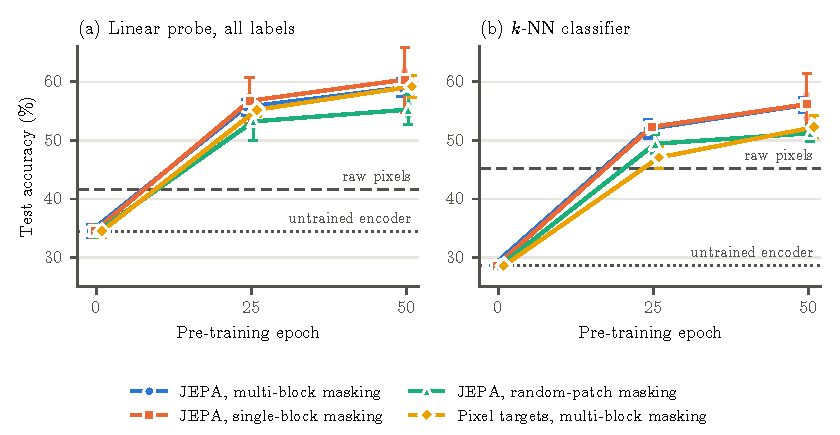
\includegraphics[width=\textwidth]{figs/fig_accuracy_vs_epoch.pdf}
\caption{Test accuracy during pre-training. Lines show the mean over three seeds with 95\% confidence intervals; dots show individual seeds (slightly offset horizontally for readability). Epoch 0 is the untrained encoder, identical for all four variants. Dashed and dotted horizontal lines show the raw-pixel classifier and the untrained encoder.}\label{fig:curves}
\end{figure}

The paired gains over the untrained encoder (Table~\ref{tab:paired}, top block) are $+24.5\pm1.1$ pp for multi-block JEPA, $+25.9\pm4.5$ for single-block, $+20.8\pm3.4$ for random-patch, and $+24.7\pm1.3$ for the pixel-target control (linear probe, all labels). All twelve intervals in this block exclude zero. The gains are similar with fewer labels: with 10\% of the labels they range from $+18.2$ to $+23.7$ pp, and with 1\% of the labels the gain for multi-block JEPA is $+18.4\pm5.0$ pp. Accuracy was still increasing between epochs 25 and 50 for every variant (linear probe: multi-block 55.7\% to 59.0\%, single block 56.7\% to 60.4\%, random patches 53.2\% to 55.2\%, pixel targets 55.2\% to 59.2\%), so the final values are not converged ones.

\needspace{14\baselineskip}
\begin{center}
\captionof{table}{Paired differences in test accuracy (percentage points, trained minus reference, same seeds) after 50 epochs, mean $\pm$ 95\% confidence interval over three seeds. Bold entries are those whose interval excludes zero. The top block shows the effect of training, the bottom block compares recipes. See also Figure~\ref{fig:paired}.}\label{tab:paired}
\resizebox{\textwidth}{!}{%
\begin{tabular}{@{}lccc@{}}
\toprule
Comparison (A $-$ B) & Linear (100\%) & Linear (10\%) & $k$-NN\\
\midrule
JEPA multi-block $-$ untrained & \textbf{$+$24.5 $\pm$ 1.1} & \textbf{$+$22.6 $\pm$ 0.7} & \textbf{$+$27.4 $\pm$ 1.0} \\
JEPA single block $-$ untrained & \textbf{$+$25.9 $\pm$ 4.5} & \textbf{$+$23.7 $\pm$ 5.7} & \textbf{$+$27.6 $\pm$ 5.0} \\
JEPA random patches $-$ untrained & \textbf{$+$20.8 $\pm$ 3.4} & \textbf{$+$18.2 $\pm$ 4.8} & \textbf{$+$22.6 $\pm$ 1.8} \\
pixel-target multi-block $-$ untrained & \textbf{$+$24.7 $\pm$ 1.3} & \textbf{$+$23.2 $\pm$ 2.8} & \textbf{$+$23.6 $\pm$ 2.4} \\
\midrule
JEPA multi-block $-$ pixel-target multi-block & $-$0.2 $\pm$ 2.4 & $-$0.5 $\pm$ 2.2 & \textbf{$+$3.8 $\pm$ 3.0} \\
JEPA multi-block $-$ JEPA single block & $-$1.4 $\pm$ 4.8 & $-$1.1 $\pm$ 5.8 & $-$0.2 $\pm$ 4.0 \\
JEPA multi-block $-$ JEPA random patches & \textbf{$+$3.7 $\pm$ 2.9} & \textbf{$+$4.5 $\pm$ 4.3} & \textbf{$+$4.8 $\pm$ 2.6} \\
JEPA single block $-$ JEPA random patches & $+$5.1 $\pm$ 7.7 & $+$5.5 $\pm$ 9.7 & $+$5.0 $\pm$ 6.5 \\
\botrule

\end{tabular}}
\end{center}

\begin{figure}[t]
\centering
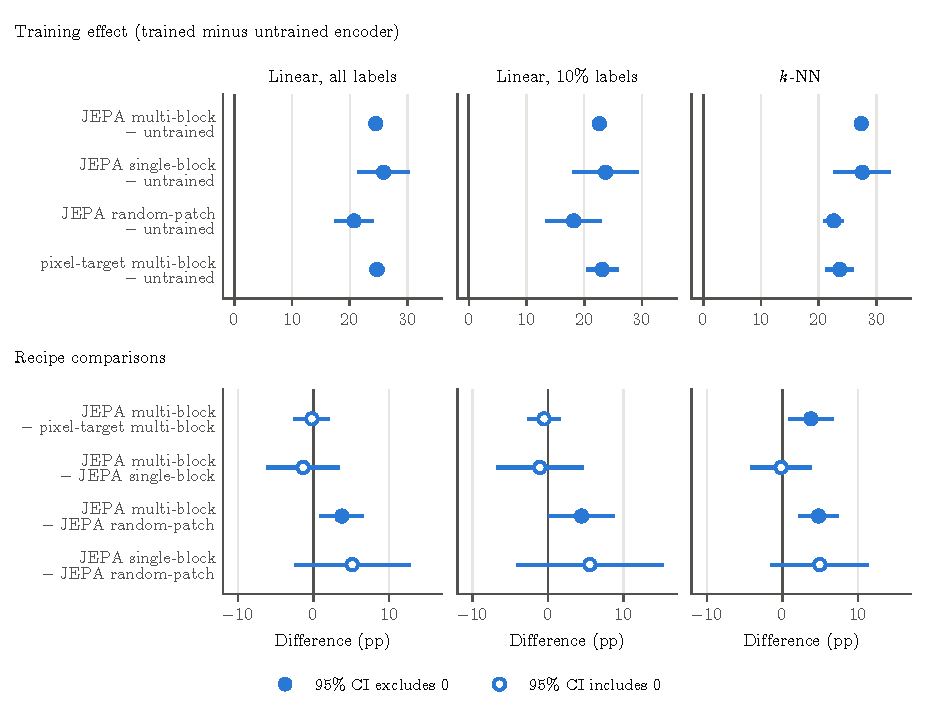
\includegraphics[width=\textwidth]{figs/fig_paired_differences.pdf}
\caption{Paired differences in percentage points (pp) with 95\% confidence intervals over three seeds, for the comparisons in Table~\ref{tab:paired}. Filled markers: the interval excludes zero. Note the different horizontal scales in the two rows.}\label{fig:paired}
\end{figure}

\subsection{Feature-space and pixel targets perform alike on the linear probe}\label{sec:res-targets}
With identical multi-block masks and predictor, feature-space targets and normalised-pixel targets give the same linear-probe accuracy: $59.0\pm1.5\%$ against $59.2\pm1.8\%$, a paired difference of $-0.2\pm2.4$ pp (Table~\ref{tab:paired}). The same holds with 10\% of the labels ($-0.5\pm2.2$) and with 1\% ($-0.9\pm4.0$). The only metric on which feature-space targets are ahead is $k$-NN accuracy ($+3.8\pm3.0$ pp, $56.0\%$ against $52.2\%$). Since this is one of 24 uncorrected comparisons, we regard it as suggestive and not as established. The two kinds of model also differ in their features: the pixel-target encoder has a lower effective rank (52.1 against 68.6).

\subsection{Masking strategy}\label{sec:res-masking}
Multi-block masking beats random-patch masking on every metric: $+3.7\pm2.9$ pp (linear, all labels), $+4.5\pm4.3$ (10\% labels), $+4.8\pm2.6$ ($k$-NN) and $+5.9\pm4.0$ (1\% labels). Single-block and multi-block masking cannot be distinguished: the difference is $-1.4\pm4.8$ pp in favour of single-block masking on the linear probe, with intervals covering zero on all metrics. Single-block masking is also the least stable recipe: the standard deviation of its linear accuracy across seeds is 2.2 pp (individual runs 61.4\%, 61.9\%, 57.8\%), against 0.6 for multi-block, 1.0 for random patches and 0.7 for pixel targets.

The cleanest comparison of target geometry is single block against random patches, since both hide 16 patches and leave 48 visible. The mean difference is $+5.1\pm7.7$ pp in favour of the contiguous block, with the interval covering zero, so the data do not establish it; the difference is, however, positive in all three seeds (7.2, 6.6 and 1.6 pp).

\subsection{Collapse and training loss}\label{sec:res-diag}
No run came close to collapse. The effective rank of the untrained encoder's features is 11.6, and all trained models are well above it (52.1 to 91.8 out of a maximum of 192). Rank does not follow accuracy across recipes: random-patch masking has the highest rank (91.8) but the lowest accuracy, and the pixel-target model has the lowest rank (52.1) but accuracy equal to multi-block JEPA. Likewise, the final training loss cannot be used to compare recipes. For feature-space targets it is 0.089 for random patches, 0.195 for single block and 0.250 for multi-block masking, and the relation to accuracy is not monotone (multi-block has the highest loss but lower accuracy than single block); the pixel-target loss (0.695) is on a different scale. Per-seed values are in Appendix~\ref{app:perseed}.

%% ------------------------------------------------------------------------------------------
\section{Discussion}\label{sec:discussion}

\paragraph{What training adds (RQ1).}
The answer is clear and robust: in this setting, training adds about 21 to 26 points of linear-probe accuracy and 23 to 28 points of $k$-NN accuracy over the untrained encoder, in every seed. The size of this number depends on the baseline. The untrained encoder with average pooling is weaker than raw pixels, so part of the gain is training recovering information that random features lose; the trained models exceed raw pixels by 14 to 19 points on the linear probe. We recommend that results of this kind be reported next to an untrained control, because without it the 55--60\% figures would suggest more learned structure than the 34.5\% reference allows.

\paragraph{Feature-space versus pixel targets (RQ2).}
In the I-JEPA paper, predicting pixels instead of target-encoder outputs lowered the 1\%-label ImageNet linear accuracy from 66.9\% to 40.7\%~\cite{assran2023ijepa}. We do not see a comparable gap: on CIFAR-10 the pixel-target control matches feature-space targets on the linear probe at all three label fractions and trails only on $k$-NN. The setups differ in many ways, and we have not tested which of them matters. Candidate explanations include the much smaller images and model, the short training schedule, and the fact that our pixel control standardises each patch, as in the normalised-pixel variant of masked autoencoders~\cite{he2022mae}, which is a stronger pixel target than raw values. The theory of Cui et al.~\cite{cui2026theory} describes a trade-off governed by latent dimension between latent-level and input-level prediction; our experiment keeps the latent dimension fixed and therefore does not test it. What our result does show is that the advantage of feature-space targets reported at large scale should not be assumed to carry over to every small-scale setting.

\paragraph{Masking (RQ3).}
Both block-based strategies scored higher than random patches (clearly so for multi-block, inconclusively for single block), and the two block-based strategies were indistinguishable. This points in the same direction as the I-JEPA ablation~\cite{assran2023ijepa}, but the effects are much smaller than the gaps of 34 and 37 points reported there between multi-block masking and single-block or random masking. The setups are not comparable (their block and random strategies hide 60\% of the patches, ours 25\%; different datasets and model sizes), so we do not read the difference in magnitude as a disagreement. Because multi-block masking changes both the geometry of the hidden regions and the amount of visible context (about 12 visible patches against 48), our comparison of multi-block with the other strategies cannot attribute its advantage over random patches to geometry. The single-block versus random comparison isolates geometry, and favours contiguous blocks, but not conclusively.

\paragraph{Limitations.}
(i)~Training is short (50 epochs) and accuracy was still rising, so the ranking of recipes could change with longer training. (ii)~Three seeds give wide, approximate intervals; several recipe differences are within noise, and the single-block recipe is notably variable. (iii)~We report 24 comparisons without correction. (iv)~One dataset, one model size and one set of hyperparameters were used, none tuned per condition; the hyperparameters follow the I-JEPA recipe and may favour the multi-block setting for which that recipe was designed. (v)~Evaluation uses average-pooled features with linear and $k$-NN classifiers only; fine-tuning or dense tasks might give other results. (vi)~Every run uses a moving-average target encoder with an annealed momentum, so we cannot say whether any condition would collapse without it. (vii)~The untrained baseline depends on the architecture and pooling choice. We have not run a literature-wide search for earlier studies of this kind (Section~\ref{sec:gap}).

\paragraph{Future work.}
Natural extensions are longer training and more seeds, a second dataset, a context-size-matched multi-block variant, a sweep over latent dimension to test the trade-off predicted by theory~\cite{cui2026theory}, ablating the moving-average target encoder, and moving from images to video, where JEPA world models are mostly used.

%% ------------------------------------------------------------------------------------------
\section{Conclusion}\label{sec:conclusion}
In a controlled, small-scale study on CIFAR-10, I-JEPA-style training raised linear-probe accuracy from 34.5\% for the untrained encoder to 55--60\%, a gain of 21 to 26 points that holds in every seed. A pixel-target control with the same masks and predictor matched feature-space targets on the linear probe, and was behind only on $k$-NN accuracy, so a large-scale advantage of feature-space targets did not appear here. Multi-block masking beat random-patch masking by about 4 points, and was indistinguishable from single-block masking. No configuration collapsed, and neither feature rank nor training loss predicted which recipe was best. These findings come from three seeds, one dataset and short training; we release the code and all results so that they can be tested at larger scale.

\bmhead{Supplementary information}
The per-seed results and the complete list of paired comparisons are provided with the code (\texttt{github.com/Amruta08/\allowbreak small-jepa-cifar10}); per-seed values are also given in Appendix~\ref{app:perseed}.

% TODO: add acknowledgements (for example, the author of the earlier Mini-JEPA experiment on which this study builds), or delete this heading.

\section*{Declarations}
\begin{itemize}
\item \textbf{Funding:} None.
\item \textbf{Conflict of interest/Competing interests:} The authors declare no competing interests.
\item \textbf{Ethics approval and consent to participate:} Not applicable.
\item \textbf{Consent for publication:} Not applicable.
\item \textbf{Data availability:} CIFAR-10 is publicly available~\cite{krizhevsky2009cifar}. The raw results of all runs (JSON files and logs), the aggregated tables and the figures are in the code repository.
\item \textbf{Materials availability:} Not applicable.
\item \textbf{Code availability:} \texttt{github.com/Amruta08/\allowbreak small-jepa-cifar10} (TODO: confirm the address once the repository is public).
\item \textbf{Author contribution:} TODO: describe each author's contribution.
\item \textbf{Use of AI tools:} An AI assistant (Claude, Anthropic) was used to help write the experiment code, analyse the results and draft the text. The authors ran the experiments and are responsible for the content. TODO: adapt this statement to your institution's policy.
\end{itemize}

%% ------------------------------------------------------------------------------------------
\begin{appendices}

\section{Hyperparameters}\label{app:hparams}
All conditions that are trained use the settings in Table~\ref{tab:hparams}.

\needspace{18\baselineskip}
\begin{center}
\captionof{table}{Training hyperparameters (identical for all trained conditions).}\label{tab:hparams}
\begin{tabular}{@{}lp{0.62\textwidth}@{}}
\toprule
Setting & Value\\
\midrule
Epochs; batch size & 50; 256 (175 steps per epoch)\\
Optimiser & AdamW~\cite{loshchilov2019adamw}, $\beta=(0.9,0.999)$\\
Learning rate & peak $10^{-3}$; 5 warm-up epochs from $10^{-4}$; cosine decay to $10^{-6}$\\
Weight decay & 0.04 increasing linearly to 0.4 (weights only; none on biases and norms)\\
Target-encoder momentum & 0.996 increasing linearly to 1.0\\
Gradient clipping & global norm 1.0\\
Precision & bfloat16 autocast; loss in 32-bit\\
Encoder & patch 4, width 192, depth 6, 3 heads, MLP ratio 4\\
Predictor & width 96, depth 4, 3 heads\\
Augmentation (pre-training) & random crop (reflection padding 4), horizontal flip\\
Train / validation / test images & 45,000 / 5,000 / 10,000\\
Linear probe & Adam, lr 0.01, cosine schedule, 300 steps, $\ell_2\in\{10^{-5},\dots,10^{-1}\}$ chosen on validation\\
$k$-NN & $k=20$, cosine similarity, temperature 0.07\\
Seeds & 0, 1, 2\\
\botrule
\end{tabular}
\end{center}

\needspace{12\baselineskip}
\section{Per-seed results}\label{app:perseed}
\setcounter{table}{0}
\begin{center}
\captionof{table}{Results of every run (test accuracy in \%; Eff.\ rank: effective rank of validation features; Loss: final-epoch training loss, which is on different scales for feature-space and pixel targets).}\label{tab:perseed}
\resizebox{\textwidth}{!}{%
\begin{tabular}{@{}lccccccc@{}}
\toprule
Condition & Seed & Lin.\ 100\% & Lin.\ 10\% & Lin.\ 1\% & $k$-NN & Eff.\ rank & Loss\\
\midrule
Raw pixels (no network) & 0 & 41.6 & 37.1 & 28.9 & 45.2 & -- & -- \\
Raw pixels (no network) & 1 & 41.7 & 37.4 & 27.8 & 45.2 & -- & -- \\
Raw pixels (no network) & 2 & 41.7 & 37.3 & 27.4 & 45.2 & -- & -- \\
\midrule
Untrained encoder & 0 & 34.6 & 33.2 & 27.8 & 28.5 & 11.4 & -- \\
Untrained encoder & 1 & 34.8 & 34.2 & 28.4 & 28.8 & 12.0 & -- \\
Untrained encoder & 2 & 34.0 & 33.2 & 27.7 & 28.5 & 11.4 & -- \\
\midrule
JEPA, multi-block & 0 & 58.6 & 56.0 & 43.9 & 56.0 & 67.7 & 0.241 \\
JEPA, multi-block & 1 & 59.7 & 56.5 & 48.1 & 56.5 & 70.7 & 0.255 \\
JEPA, multi-block & 2 & 58.6 & 56.0 & 47.1 & 55.5 & 67.3 & 0.255 \\
\midrule
JEPA, single block & 0 & 61.4 & 59.0 & 46.7 & 56.9 & 79.9 & 0.212 \\
JEPA, single block & 1 & 61.9 & 58.2 & 48.0 & 57.8 & 89.2 & 0.220 \\
JEPA, single block & 2 & 57.8 & 54.5 & 42.9 & 53.8 & 88.7 & 0.152 \\
\midrule
JEPA, random patches & 0 & 54.2 & 51.0 & 39.4 & 51.3 & 91.7 & 0.081 \\
JEPA, random patches & 1 & 55.3 & 50.6 & 40.4 & 50.6 & 90.3 & 0.097 \\
JEPA, random patches & 2 & 56.2 & 53.5 & 41.7 & 51.7 & 93.6 & 0.088 \\
\midrule
Pixel targets, multi-block & 0 & 59.9 & 57.4 & 46.4 & 52.9 & 53.1 & 0.693 \\
Pixel targets, multi-block & 1 & 59.2 & 56.2 & 47.4 & 51.4 & 51.8 & 0.697 \\
Pixel targets, multi-block & 2 & 58.5 & 56.4 & 48.0 & 52.4 & 51.2 & 0.694 \\
\botrule

\end{tabular}}
\end{center}

\end{appendices}

\bibliography{sn-bibliography}% common bib file

\end{document}
